% This file contains ONLY the content for Quiz 1
% NO preamble, NO \begin{document}, etc.

\section{Quiz 1: Bayesian Classifier for Image Segmentation}

\subsection{Objective}
The goal of this assignment is to implement a Bayesian classifier to segment an image of a cheetah from its background (grass). The classification is based on features derived from the Discrete Cosine Transform (DCT) of 8x8 image blocks.

\subsection{Methodology and Results}

\subsubsection{Part (a): Prior Probabilities}
The prior probabilities, $P(Y=\text{cheetah})$ and $P(Y=\text{grass})$, were estimated from the proportions of foreground (FG) and background (BG) samples in the provided training data, \texttt{TrainingSamplesDCT\_8.mat}. The estimation is based on the formula:
$$
P(Y=c) = \frac{N_c}{N_{\text{total}}}
$$
where $N_c$ is the number of samples for class $c$ and $N_{\text{total}}$ is the total number of training samples. Based on the 250 foreground samples and 1053 background samples, the calculated priors are as follows:
\begin{itemize}
    \item $P(Y=\text{cheetah}) = \frac{250}{250 + 1053} \approx 0.1919$
    \item $P(Y=\text{grass}) = \frac{1053}{250 + 1053} \approx 0.8081$
\end{itemize}

\subsubsection{Part (b): Class-Conditional Probabilities (Likelihoods)}
The feature used for classification is the index (from 1 to 64, following a zig-zag scan) of the DCT coefficient with the second-largest absolute value. The class-conditional probabilities, $P(X|Y)$, were estimated by creating a normalized histogram of these features for each class. The resulting probability mass functions (PMFs) are shown in Figure \ref{fig:hw1_likelihoods}. The plots show that for the cheetah class, the energy is concentrated in lower-frequency DCT coefficients (smaller indices), whereas for the grass class, the energy is more distributed towards higher-frequency coefficients.

\begin{figure}[h!]
    \centering
    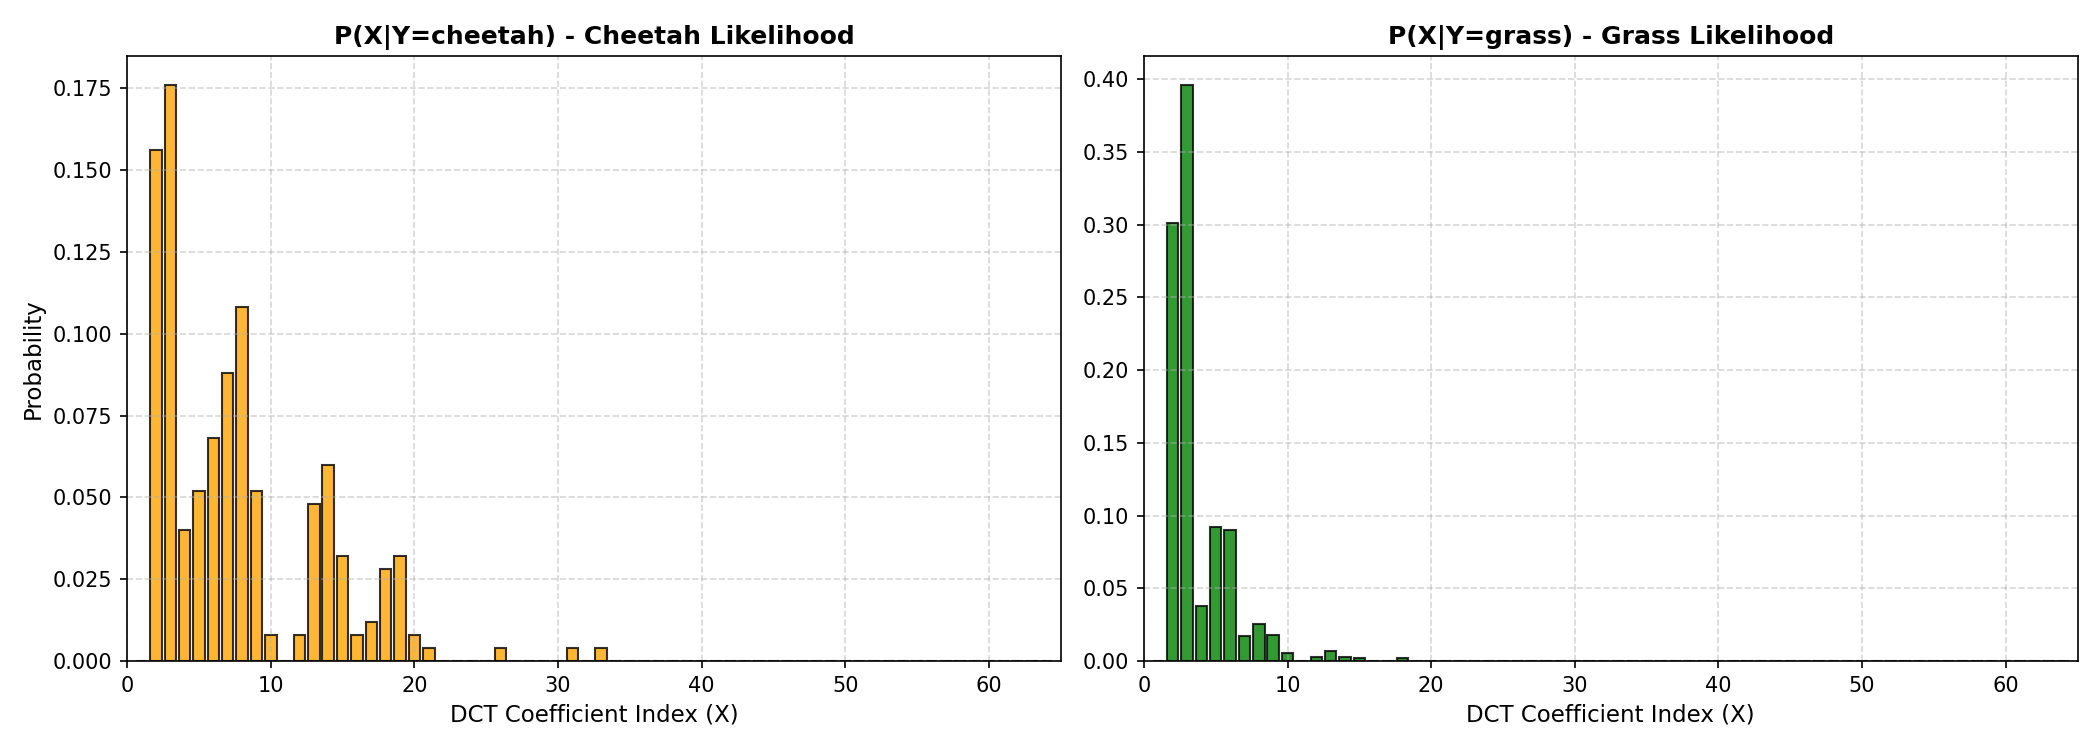
\includegraphics[width=1.0\textwidth]{hw1_likelihoods.png}
    \caption{Estimated likelihoods $P(X|Y)$ for the Cheetah (left) and Grass (right) classes.}
    \label{fig:hw1_likelihoods}
\end{figure}

\subsubsection{Part (c) \& (d): Image Segmentation and Error Rate}
The cheetah image was processed using a sliding 8x8 window. For each block, the feature was extracted and classified using the minimum probability of error rule: $\hat{Y} = \arg\max_{Y} P(X|Y)P(Y)$. The resulting segmentation mask is compared with the ground truth in Figure \ref{fig:hw1_segmentation}.

The probability of error was calculated by comparing the generated mask with the ground truth mask pixel by pixel. The formula used is:
$$
P(\text{error}) = \frac{\text{Number of Mismatched Pixels}}{\text{Total Number of Pixels}}
$$
The final computed probability of error, based on 11,566 mismatched pixels out of a total of 68,850, is: $\mathbf{16.80\%}$.

\begin{figure}[h!]
    \centering
    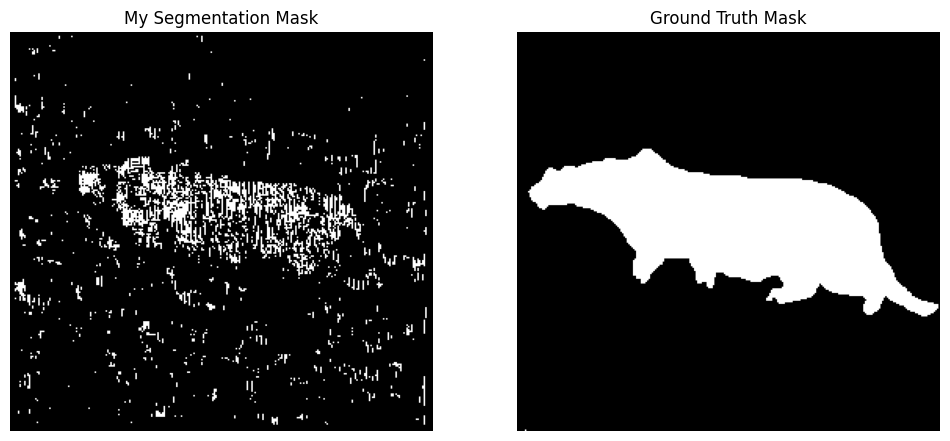
\includegraphics[width=0.9\textwidth]{hw1_segmentation.png}
    \caption{Left: Generated segmentation mask. Right: Ground truth mask.}
    \label{fig:hw1_segmentation}
\end{figure}

\newpage
\subsection{Appendix: Source Code}
The source code used for this assignment is attached below.

\begin{lstlisting}[language=Python, caption={Python code for HW1}, label={code:hw1}]
import numpy as np
from scipy.io import loadmat
from scipy.fft import dctn
import imageio.v2 as imageio
import matplotlib.pyplot as plt

# --- 1. Data Loading ---
training_data = loadmat('TrainingSamplesDCT_8.mat')
TrainsampleDCT_FG = training_data['TrainsampleDCT_FG']
TrainsampleDCT_BG = training_data['TrainsampleDCT_BG']
zigzag_pattern = np.loadtxt('Zig-Zag Pattern.txt', dtype=int)
image = imageio.imread('cheetah.bmp', pilmode='L')
mask_true = imageio.imread('cheetah_mask.bmp')

# --- 2. Part (a): Estimate Prior Probabilities ---
n_fg = TrainsampleDCT_FG.shape[0]
n_bg = TrainsampleDCT_BG.shape[0]
n_total = n_fg + n_bg
prior_cheetah = n_fg / n_total
prior_grass = n_bg / n_total

print(f"Prior P(Y=cheetah): {prior_cheetah:.4f}")
print(f"Prior P(Y=grass):   {prior_grass:.4f}")

# --- 3. Part (b): Estimate Class-Conditional Probabilities ---
def extract_features(data):
    """Extracts the index of the 2nd largest absolute value for each sample."""
    abs_data = np.abs(data)
    sorted_indices = np.argsort(abs_data, axis=1)[:, ::-1]
    # Return the second column (index of 2nd largest value) + 1 for 1-based indexing
    return sorted_indices[:, 1] + 1

features_fg = extract_features(TrainsampleDCT_FG)
features_bg = extract_features(TrainsampleDCT_BG)

bins = np.arange(1, 66)
hist_fg, _ = np.histogram(features_fg, bins=bins)
hist_bg, _ = np.histogram(features_bg, bins=bins)

likelihood_cheetah = hist_fg / n_fg
likelihood_grass = hist_bg / n_bg

# --- 4. Part (c): Classify the Image ---
image_float = image.astype(np.float64) / 255.0
height, width = image.shape
block_size = 8
segmentation_mask = np.zeros((height - block_size + 1, width - block_size + 1))

zigzag_flat = zigzag_pattern.flatten()
inverse_zigzag = np.empty_like(zigzag_flat)
inverse_zigzag[zigzag_flat] = np.arange(len(zigzag_flat))

for i in range(height - block_size + 1):
    for j in range(width - block_size + 1):
        block = image_float[i:i+block_size, j:j+block_size]
        dct_block = dctn(block, type=2, norm='ortho')
        dct_vector = dct_block.flatten()[inverse_zigzag]

        feature_idx_0based = np.argsort(np.abs(dct_vector))[::-1][1]
        feature = feature_idx_0based + 1

        # Apply Bayes Decision Rule using log-posteriors to avoid underflow
        epsilon = 1e-10
        posterior_cheetah = np.log(prior_cheetah) + np.log(likelihood_cheetah[feature - 1] + epsilon)
        posterior_grass = np.log(prior_grass) + np.log(likelihood_grass[feature - 1] + epsilon)

        if posterior_cheetah > posterior_grass:
            segmentation_mask[i, j] = 1 # 1 for cheetah
        else:
            segmentation_mask[i, j] = 0 # 0 for grass

# --- 5. Part (d): Compute Probability of Error ---
mask_true_binary = (mask_true / 255).astype(int)

mismatched_pixels = np.sum(segmentation_mask.astype(int) != mask_true_binary)
total_pixels = mask_true_binary.size
error_rate = mismatched_pixels / total_pixels

print(f"Total pixels: {total_pixels}")
print(f"Mismatched pixels: {mismatched_pixels}")
print(f"Probability of Error: {error_rate:.4f} or {error_rate * 100:.2f}%")
\end{lstlisting}